\documentclass[]{article}
\usepackage[backend=biber, style=numeric]{biblatex}
\usepackage{paralist}
\usepackage{hyperref}
\usepackage{float}
\usepackage{graphicx}
\usepackage{booktabs}
\usepackage[margin=2.5cm]{geometry}
\graphicspath{ {./images/} }

\addbibresource{report.bib}
\newtheorem{researchquestion}{RQ}

%opening
\title{A YOLOv8-based Analysis of Image Augmentation Techniques for Vehicle Detection in Adverse Weather Conditions}
	\author{
		Alexander Van Hecke \small(852631385) \and 
		Frederik Lefever    \small(838836963)}

\begin{document}

\maketitle

\begin{abstract}
	Vehicle detection is an important aspect of semi-automated traffic monitoring and surveillance.  We investigate whether the technique of image augmentation can be used to increase the accuracy of vehicle detection in adverse weather conditions.  We evaluate whether the use of image augmentation to train a YOLO\small{v8} model increases accuracy compared to a baseline model.  We also compare the effect of training with augmentated images to that of training with actual images of traffic in adverse weather conditions. To this extent we train a YOLO\small{v8} model with actual adverse weather images and compare with the same baseline model and the accuracy obtained from the first model. Our main hypothesis is that image augmentation can indeed be used to improve the accuracy of vehicle detection in adverse weather conditions. Our secondary hypothesis is that the accuracy of a model derived from augmented images falls within statistically insignificant margins when compared to a model obtained from actual images.
\end{abstract}

\section{Introduction}

	Adverse weather conditions such as rainfall, snow and fog are widely considered to have an effect on traffic flow. Traffic breakdown occurs when demand exceeds capacity in some part of a transportation network and in \cite{stralenInfluenceAdverseWeather2015} it is shown that the odds of traffic breakdown at bottleneck locations are significantly increased by rainfall.  This can lead to considerable economic damage and provides a strong incentive to mitigate this problem as much as possible.
	
	Traffic monitoring and dynamic flow control can be part of a mitigation strategy. The current technology behind traffic monitoring largely uses vehicle detection in images captured from CCTV cameras positioned next to highways. However, vehicle detection in images can be influenced by adverse weather conditions.
	
	We investigate the effect of image augmentation on the robustness of YOLO{\small v8}-based vehicle detection models. In particular, we investigate the effect of artificially adding rain, fog and snow to clear weather images of traffic situations. Compared to the standard YOLO{\small v8} model, we expect to see an improvement of the Mean Average Precision (mAP) for vehicle detection in models derived from YOLO{\small v8} by training on the augmented images. YOLO{\small v8} was chosen because it is popular in both academia and industry, and is well-documented, both as a ready-to-use product and in scientific literature. Finally, YOLO{\small v8} is an open-source software, licensed under AGPL-3.0.  All artifacts produced by the study will be made available through a public GitHub repository.

\section{Literature review}

	In the context of machine learning, image augmentation can broadly be defined as the automated creation of variation in actual image datasets. Large volumes of data with sufficient variation can alleviate the problem of overfitting. Yet sometimes sampling data from an application domain is nontrivial, eg. when learning from medical images.  Image augmentation can be used to artificially create additional images, or to add some sort of noise to images in order to make the resulting model more robust.
	
	A comprehensive survey of modern image augmentation techniques is presented in \cite{shortenSurveyImageData2019}. Several approaches such as geometric transformations, color space augmentations, kernel filters, mixing images, random erasing, feature space augmentation, adversarial training, generative adversarial networks, neural style transfer, and meta-learning, are explained.  A more recent survey of image augmentation techniques as used in deep learning is presented in \cite{xuComprehensiveSurveyImage2023} . This survey introduces a novel taxonomy, where image augmentation algorithms are classified as either model-free, model-based, or optimizing policy-based. The objectives of image augmentation are explained by analyzing the challenges encountered when deploying deep learning models for computer vision. A theoretical framework for understanding data augmentation is described in \cite{daoKernelTheoryModern2019}. First a general model of augmentation as a Markov process is given, and it is shown that kernels appear naturally with respect to this model. Next, a more direct analysis of the effect of augmentation on kernel classifiers is offered.
	
	The effectiveness of image augmentation on the classification of images with deep learning is discussed in \cite{perezEffectivenessDataAugmentation2017}. Simple techniques, such as cropping, rotating, and flipping images are compared. Additionally this paper reports on experiments with generative adversarial neural networks to learn augmentation strategies.
	
	Research similar to our research can be found in \cite{kumarObjectDetectionAdverse2023}. The central question in \cite{kumarObjectDetectionAdverse2023} is whether YOLO{\small v8} can be improved through transfer learning to detect objects in adverse weather. This paper supports the hypothesis that training with actual images of adverse weather conditions significantly improves the detection performance compared to the standard YOLO{\small v8} model. An enhanced YOLO\small{v8}-based model for vehicle detection in foggy weather conditions is the focus of \cite{liVehicleDetectionFoggy2022}. The approach used to create the enhanced model is interesting in that the trainingset is obtained from 350 traffic images that are augmented with a fog-effect and subsequently dehazed with the multi-scale retinex with color restoration (MSRCR) algorithm. The final trainingset is then composed of the original images, fogged images and dehazed images. Whereas results in \cite{liVehicleDetectionFoggy2022} are reported with autonomous vehicles in mind, \cite{songVisionbasedVehicleDetection2019} specifically targets vehicle detection and counting in highway management.  A new segmentation method is proposed to divide a depicted highway road surface into a distal and a proximal area. Using this separation a YOLO{\small v3} model is trained to detect the type and location of vehicles. To estimate vehicle count and trajectories the Oriented FAST and Rotated BRIEF (ORB) algorithm is added to the image processing pipeline.
	

\section{Research questions}

	Many image augmentation techniques are described in literature, ranging from simple geometric transformations to the addition of noise and the changing of color, saturation and hue parameters. We investigate the effect of \textit{thematic} image augmentation, meaning we will artificially add rain, fog and snow to clear weather images. At the more general level, we aim to answer following questions:

	\begin{researchquestion}
		\label{rq1}
		Will a YOLO{\small v8} model trained with thematically augmented images be more accurate (measured by the mean average precision (mAp) at 0.50-0.95 IoU) in predicting the location of vehicles in adverse weather images than the baseline large YOLO{\small v8} model?
	\end{researchquestion}

	Furthermore, to appreciate the value of image augmentation in contexts where data is not necessarily scarce, we pose two additional questions:
	\begin{researchquestion}
		\label{rq2}
		Will a YOLO{\small v8} model trained with adverse weather images be more accurate (measured by the mean average precision (mAp) at 0.50-0.95 IoU) in predicting the location of vehicles in adverse weather images than the baseline large YOLO{\small v8} model?
	\end{researchquestion}

	\begin{researchquestion}
		\label{rq3}
		Will a YOLO{\small v8} model trained with adverse weather images be as accurate as (measured by the mean average precision (mAp) at 0.50-0.95 IoU) a YOLO{\small v8} model trained with thematically augmented images in predicting the location of vehicles in adverse weather images?
	\end{researchquestion}

\section{Research method}
\subsection{Measuring model accuracy}

	To estimate the robustness of vehicle detection models, we use the mean average precision (mAP) at 0.50-0.95 IoU, henceforth simply referred to as ``mAP''. The mAP is an aggregate metric based on the confusion matrix, the intersection over union (IoU), recall and precision. In this study, we only consider two relevant classes of vehicles, namely ``car'' and ``bus''.

\subsubsection{Calculation of the mAP at 0.50-0.95 IoU}

	The mAP is calculated by dividing the sum of the average precision ($AP$) per class by the number of classes $N$.  In our study $N = 2$ (``car'' and ``bus'').
	
	\[
	mAP = \frac{1}{N} \sum_{i=1}^{N} AP_i
	\]

	The $AP$ of a model is obtained by the following steps:

	\begin{center}
		\begin{compactenum}
			\item Use model to generate prediction scores
			\item Map prediction scores onto class labels
			\item Construct the confusion matrix
			\item Calculate precision and recall for a set of IoU thresholds (0.50-0.95)
			\item Calculate area under precision-recall curve
			\item Calculate average precision
		\end{compactenum}
	\end{center}

	The IoU metric is used to evaluate the performance of object detection by quantifying the fit between the ground truth bounding box and the predicted bounding box.
	
	\begin{figure}[h]
		\centering
		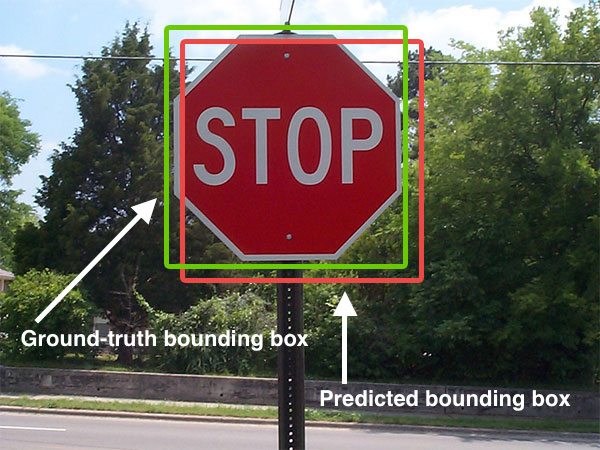
\includegraphics[width=5cm]{Intersection_over_Union_-_object_detection_bounding_boxes.jpg}
		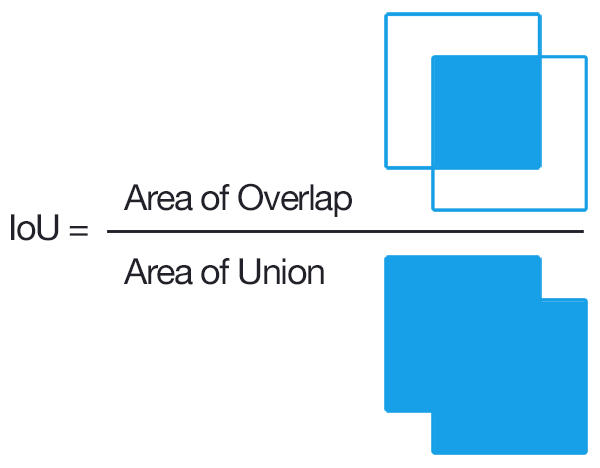
\includegraphics[width=5cm]{Intersection_over_Union_-_visual_equation.png}
		\caption{Images from Wikipedia \footnotesize{(\url{https://en.wikipedia.org/wiki/Jaccard_index})}}
	\end{figure}
	
	By using a lower bound for the value of the IoU metric, one can discriminate between positive and negative predictions. The IoU metric can then be used to calculate recall and precision. In the context of traffic management, it seems reasonable to slightly favour recall over precision and choose an IoU threshold to reflect this preference. However, choosing a good IoU threshold is itself an optimization process. For comparing models, optimizing the IoU threshold is unnecessary. Instead, we calculate AP as an average of AP's calculated for a set of IoU thresholds per class.

\subsection{Datasets}

	Two open-source datasets are used for this research. The DAWN dataset \cite{bw1x-yh39-20} is a collection of 1000 images from real-traffic environments in adverse weather conditions. The images are divided into four sets of weather conditions: fog, snow, rain and sandstorms. They are annotated with object bounding boxes and are labelled.  The second dataset is the UA-DETRAC \cite{CVIU_UA-DETRAC} dataset. This dataset provides 140K traffic images taken at Beijing and Tianjin (China). Images of the UA-DETRAC dataset are divided into four weather categories: ``cloudy'', ``night'', ``sunny'' and ``rainy''. They are annotated with object bounding boxes and are labelled.  We focused on the common labels between these two datasets, ``car'' and ``bus''.

\subsection{Model selection}
 
	For vehicle detection we chose an open source convolutional neural network called YOLO{\small v8} \cite{yolov8_ultralytics}. We use this model in transfer learning and as a reference for derived models. YOLO{\small v8} is trained on the Microsoft COCO dataset \cite{linMicrosoftCOCOCommon2015a} and capable of detecting object categories ``car'' and ``bus''.  Several sizes of the YOLO{\small v8} model are available, ranging from a ``nano'' model to a ``large'' model.  We started from the ``large'' model in all experiments, and trained it for 300 epochs.  This is the minimum number of epochs suggested by the authors of the YOLO{\small v8} model.

\subsection{Experiments}

From the DAWN dataset, only images containing at least one of the common labels (``car'', ``bus'') were kept.  Sandstorm images were not kept, as this was not something we could artificially generate using the chosen augmentation software imgaug \cite{imgaug} (version 0.4.0).  This resulted in 698 images, which were first shuffled randomly and then split in a training set of 501 images (about 70\%), a validation set of 99 images (about 15\%), and a test set of 98 images (about 15\%).

From the UA-DETRAC dataset, only images taken in sunny conditions were kept.  As the goal was to artificially augment these images, we wanted to start from the best weather condition possible.  These images were shuffled randomly and a selection of 167 training images and 33 validation was made.  Each of those images was then artificially augmented with a fog effect, a snow effect (flake size $[0.8 - 1.0]$, speed $[0.01 - 0.05]$), and a rain effect (drop size $[0.4 - 0.8]$, speed $[0.3 - 0.8]$).  This resulted in a training set of $3 \times 167=501$ images, and a test set of $3 \times 33=99$ validation images, the same number of images as in the training and validation sets of the DAWN dataset.  See Table \ref{table:datasets} for an overview, and Figure \ref{fig:example-images} for examples of images from the DAWN and UA-DETRAC datasets (both with and without augmentation).

\begin{table}[H]
	\centering
	\begin{tabular}{cccrrrp{1.5in}}
		\toprule
		\textbf{dataset} & \textbf{relevant labels} & \textbf{filter} & \textbf{training} & \textbf{validation} & \textbf{test} \\
		\midrule
		\textbf{DAWN} & car, bus & fog, snow, rain & 501 & 99 & 98  \\
		\textbf{UA-DETRAC} & car, bus & sunny &  501 & 99 &  \\
		\bottomrule
	\end{tabular}
	\caption{Datasets used}
	\label{table:datasets}
\end{table}

\begin{figure}
	\begin{tabular}{cc}
		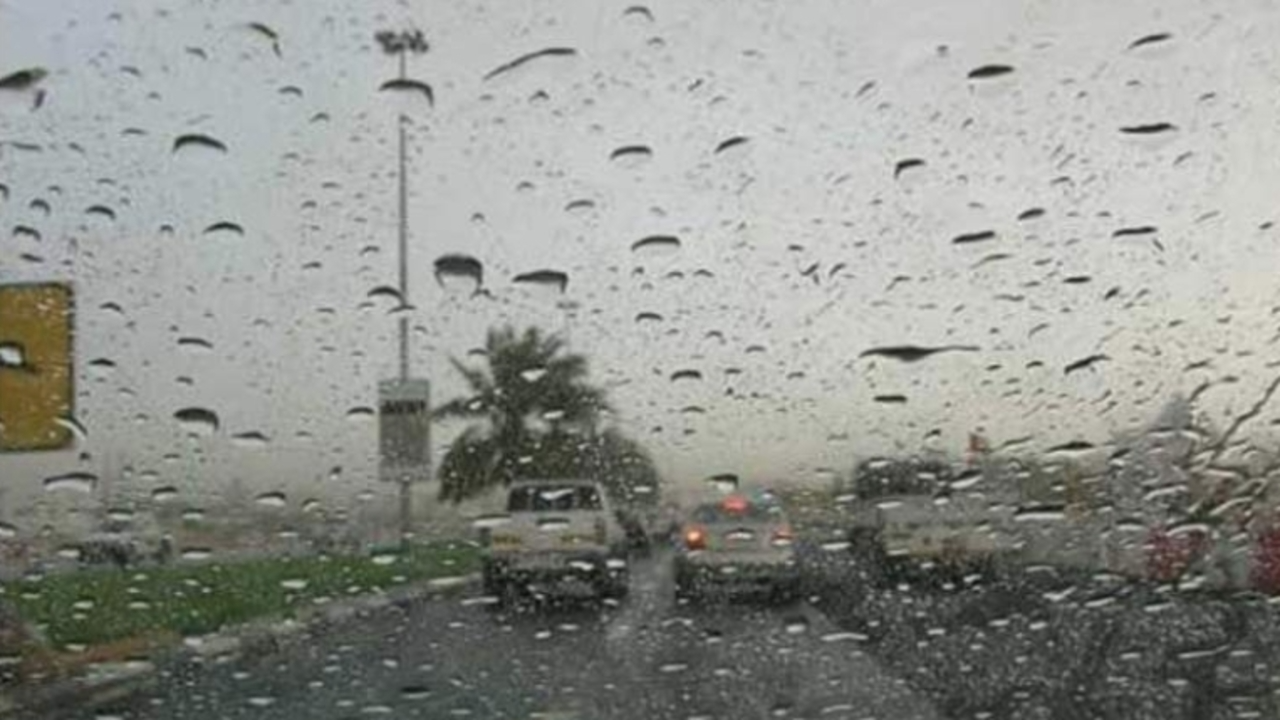
\includegraphics[width=65mm, height=40mm]{dawn-train-fullres.png} &   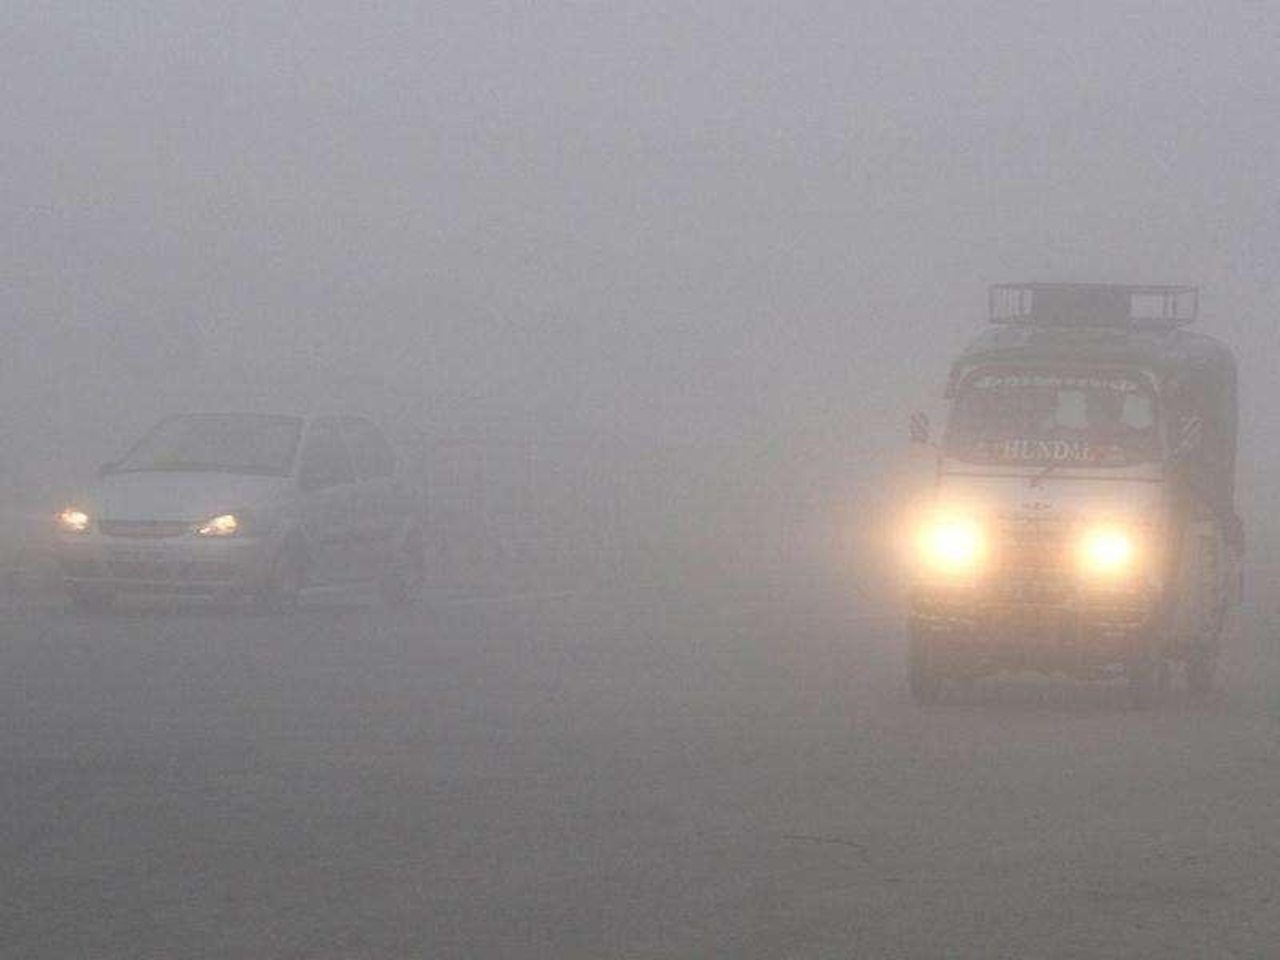
\includegraphics[width=65mm, height=40mm]{dawn-fog.jpg} \\
		(a) DAWN rain & (b) DAWN fog  \\[6pt]
		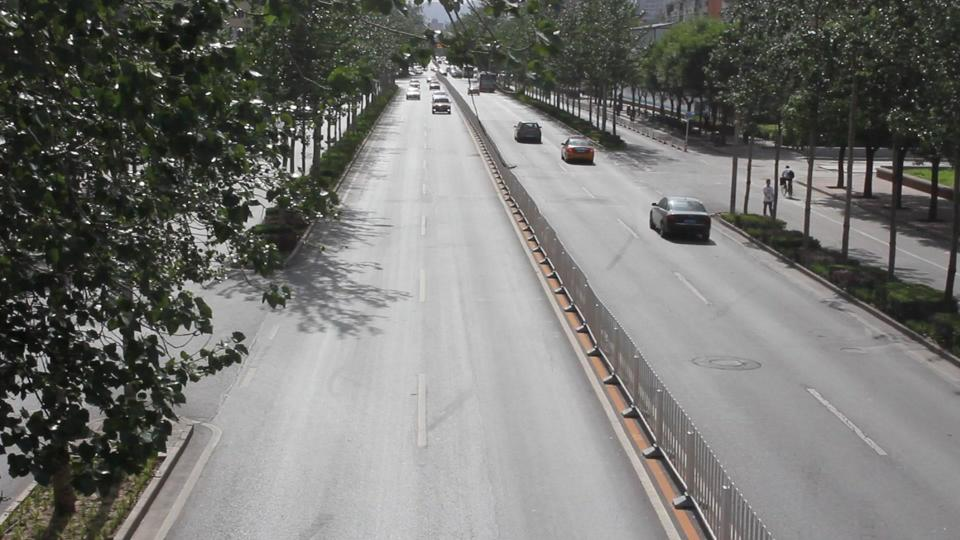
\includegraphics[width=65mm, height=40mm]{detrac-orig.jpg} &   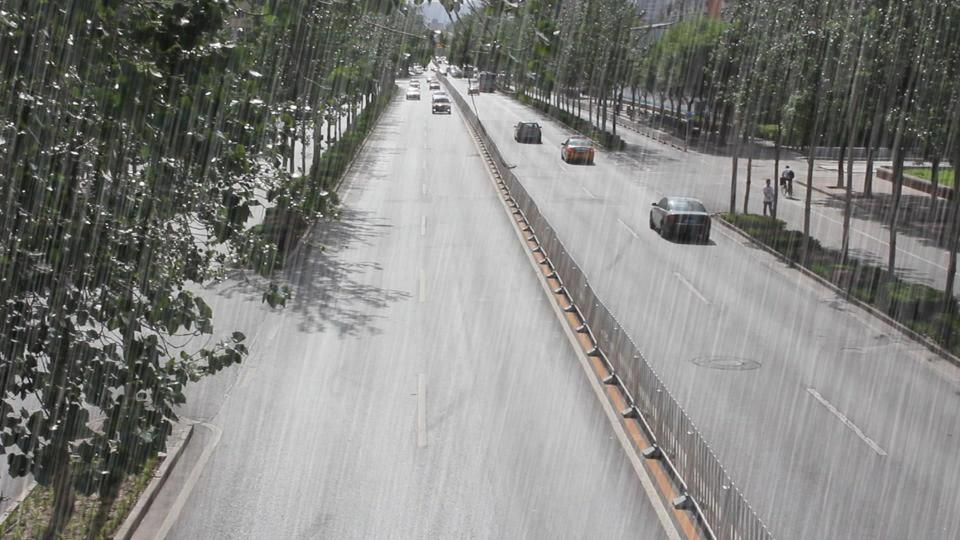
\includegraphics[width=65mm, height=40mm]{detrac-rain-fullres.png} \\
		(c) UA-DETRAC original  & (d) UA-DETRAC augmented rain \\[6pt]
		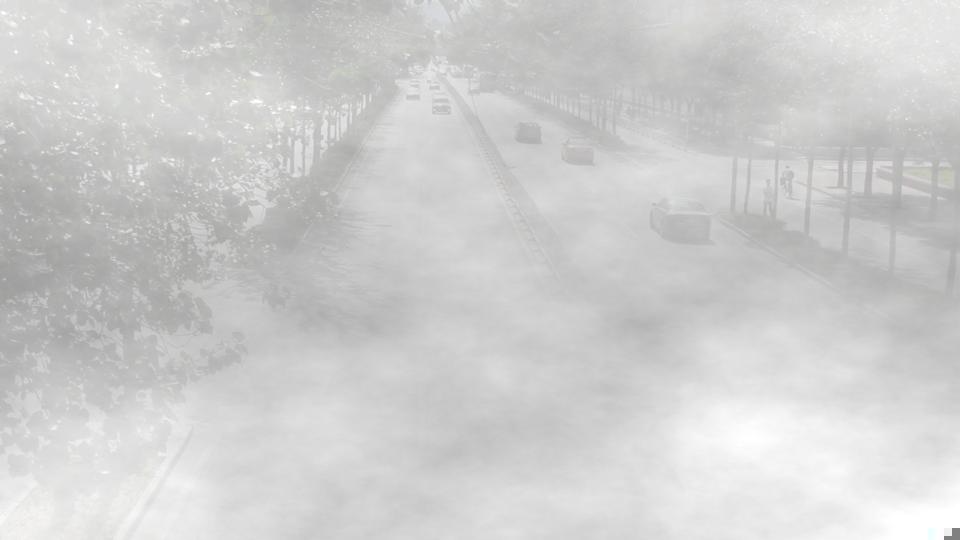
\includegraphics[width=65mm, height=40mm]{detrac-fog-fullres.png} &   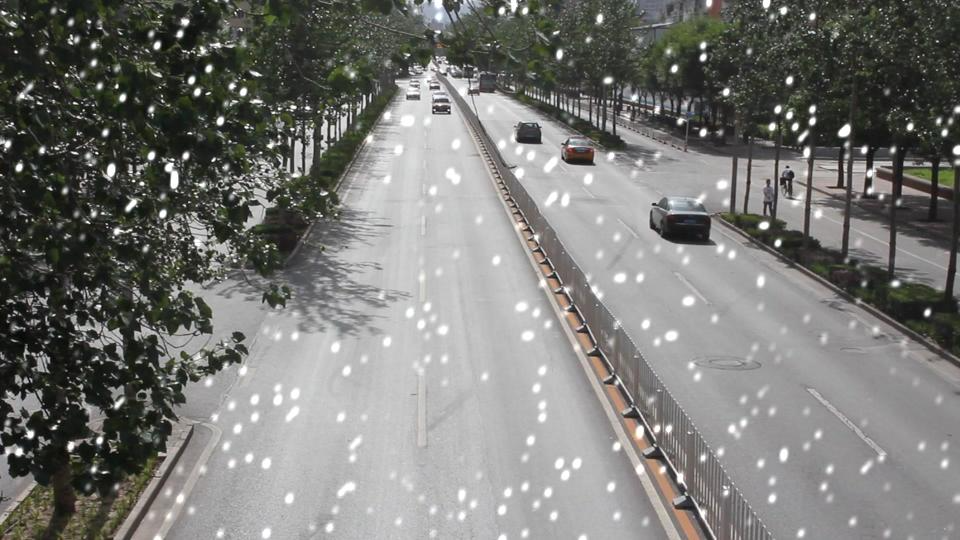
\includegraphics[width=65mm, height=40mm]{detrac-snow-fullres.png} \\
		(c) UA-DETRAC augmented fog & (d) UA-DETRAC augmented snow \\[6pt]
	\end{tabular}
	\caption{Example images of the DAWN and UA-DETRAC datasets.  (a) contains a rainy image in the DAWN dataset, (b) a foggy image in the DAWN dataset.  (c) contains an original image in the UA-DETRAC dataset (sunny conditions).  This UA-DETRAC image is artificially augmented with rain (d), fog (e) and snow (f)  }
	\label{fig:example-images}
\end{figure}

To establish a baseline measurement, we took the out-of-the-box large YOLO{\small v8} model and used it to do predictions against the test dataset taken from DAWN (adverse weather images).  To answer the first research question \ref{rq1}, we trained a large YOLO{\small v8} model using the training and validation dataset taken from UA-DETRAC (augmented images) for 300 epochs.  This model was used to do predictions against the test dataset taken from DAWN (adverse weather images).  To answer the second research question \ref{rq2}, we trained a large YOLO{\small v8} model using the training and validation dataset taken from DAWN (adverse weather images) for 300 epochs.  This model was used to do predictions against the test dataset taken from DAWN (adverse weather images).  This is summarized in Table \ref{table:setuprq}.

\begin{table}[H]
	\centering
	\begin{tabular}{lll}
		\toprule
		\textbf{research question} & \textbf{training and validation} & \textbf{test} \\
		\midrule
		RQ1 & UA-DETRAC (thematically augmented images) & DAWN (adverse weather images) \\
		RQ2 & DAWN (adverse weather images) & DAWN (adverse weather images) \\
		\bottomrule
	\end{tabular}
	\caption{setup RQ \ref{rq1}}
	\label{table:setuprq}
\end{table}
\section{Data analysis}

	Our approach to the proposed study will be that of a single case mechanism experiment. More specifically, we investigate the effect of differences in an independent variable $X$ being a model derived from transfer learning, on a dependent variable $Y$ being the mean average precision. Since we only consider three models (standard YOLO{\small v8}, a model derived from augmented images and a model derived from actual images), the study does not produce a volume of data large enough to use statistical inference.
	
	Our scientific hypothesis related to research question \ref{rq1} is that, for the detection of cars and busses in images of traffic in adverse weather conditions, the mAP at 0.50-0.95 IoU of a model obtained by transfer learning from the standard YOLO{\small v8} with thematically augmented images, is higher than the mAP at at 0.50-0.95 IoU of the standard YOLO{\small v8}. 	
	
	Related to research question \ref{rq2}, our scientific hypothesis is similar to the hypothesis related to research question \ref{rq1}. Ie, for the detection of cars and busses in images of traffic in adverse weather conditions, the mAP at 0.50-0.95 IoU of a model obtained by transfer learning from the standard YOLO{\small v8} with  \textit{actual} images, is higher than the mAP at 0.50-0.95 IoU of the standard YOLO{\small v8}.  
	
	The statistical significance of the observed differences in accuracy must be left undecided in this study. Yet we will attempt to give an explanation of the causal relationship between image augmentation and improved accuracy of prediction.
	
	To conclusively answer research question \ref{rq3} in which we compare the accuracy of a model learned from augmented images with that of a model learned from actual images, the design of our study cannot provide sufficient evidence. Nevertheless, we will shortly present our intuitions based on our understanding of neural networks.
	
	Finally, by brief consideration of the learnability properties of other base models we should be able to generalize our findings by analogy with YOLO{\small v8}.	

\section{Conclusion}

TODO TODO

\printbibliography

\end{document}
